In diesem Abschnitt sollen vorranging grundlegende Arten von Motion Sickness erkl\"art und gegen\"uber gestellt sowie Theorien zur Entstehung dieser vorgestellt werden. Au{\ss}erdem soll wird darauf verwiesen werden, welche Probleme das f\"ur Virtual Reality impliziert.

Das gravierendste Problem, welches bei der Nutzung von Virtual Reality auftreten kann, sind die Symptome der Cyber Sickness. Diese \"ahneln denen der klassischen Motion Sickness und umfassen eine Vielzahl unangenehmer Empfindungen und Reaktionen durch den betroffenen Organismus: Kopfschmerzen, Schwei{\ss}ausbr\"uche, Orientierungslosigkeit, Schwindelanf\"alle, Ataxia und \"Ubelkeit bis hin zum Erbrechen\cite{LaViola:2000:CSinVR, Kolasinski:1998:SympCS}.

Durch die \"Ahnlichkeit in den k\"orperlichen Reaktionen zur klassischen Motion Sickness, die beispielsweise von Auto- oder Schifffahrten bekannt ist, versucht man auch, denselben Erkl\"arungsansatz zu verwenden: die \textit{Sensory Conflict Theory}\cite{Kolasinski:1998:SympCS,Johnson:2005:SCT_Expl}.
Diese postuliert, dass die eben genannten Symptome auftreten, wenn bei der multimodalen, sensorischen Integration\footnote{ Verarbeitung der Reize verschiedener Sinneskan\"ale auf h\"oheren kognitiven Ebenen} bez\"uglich der Selbstbewegung inkongruente Reize festgestellt wurden und vor allem dann, wenn die aktuelle Wahrnehmung im Widerspruch mit vorherigen Lernerfahrung in \"ahnlichen Situationen steht\cite{Reason:1975:MSexp}.

Ein m\"oglicher Grund, warum manche der Symptome auftreten, k\"onnte laut Treisman\cite{Treisman:1977:Toxic} ein evolution\"arer Schutzmechanismus vor Vergiftung sein. Leider bietet diese Theorie wenig M\"oglichkeiten zur Pr\"adiktion.

F\"ur die Wahrnehmung von Bewegung ist die Propriozeption, vor allem aber der Gleichgewichtssinn und Sehsinn zust\"andig.
Bei klassicher Motion Sickness besteht das Problem darin, dass keine visuellen Reize vorhanden sind, wie auf der Innenkabine eines Schiffes bei starkem Wellengang, was bekannterma{\ss}en zu Seekrankheit, eine Form der Motion Sickness, f\"uhrt.

Im Gegensatz dazu entsteht bei Virtual Reality \textit{Vection}\footnote{ Illusion in der Wahrnehmung der Eigenbewegung} allein durch visuelle Stimuli, ohne das Vorhandensein von vestibul\"aren Reizen.
Zwar ist es Ziel der Virtual Reality, eine Vection zu erzeugen, sodass sie immersiv ist und ein Entstehen von Presence gelingt, jedoch ist das mit Virtual Reality Sickness\footnote{Synonym f\"ur Cyber Sickness} negativ korreliert, wie Weech at al.\cite{Weech:2019:PresenceCS} in ihrer Metaanalyse herausfanden (\autoref{abb:presence_vrsick}).

Bei beiden, klassicher Motion und Cyber Sickness, liegt der \textit{visuell-vestibul\"are Konflikt} zu Grunde, jedoch ist die Art, wie dieser entsteht, ebenso wie einige Symptome der beiden, unterschiedlich \cite{Stanney:1997:MSCSSS}. Deswegen wird die Sensory Conflict Theory auch teils als Erkl\"arung f\"ur die Symptome der Virtual Reality Sickness angezweifelt  \cite{Kolasinski:1998:SympCS}. Dennoch l\"asst sich ihrer Hilfe gut erkl\"aren, warum die Ma{\ss}nahmen gegen Cyber Sickness in  \autoref{Maßnahmen gegen CS} helfen.

Durch die Symptome kann sich eine Aversion gegenüber Virtual Reality entwickeln und im Falle von Trainingsszenarien in virtuellen Umgebungung, wenn die Teilnehmer das Szenario nicht freiwillig beenden können, kann es vorkommen, dass ein unerwünschtes Vermeidungsverhalten, wie Passivit\"at, gefestigt wird\cite{Crowley:1987:Avoid}, welches sich kontraproduktiv auswirken könnte, wenn der Realfall des Trainingsszenario eintritt.




\begin{figure}[bt]
	\centering 
	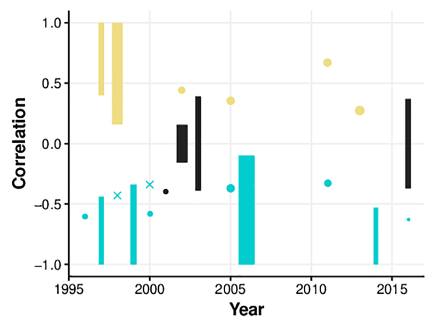
\includegraphics[width=\columnwidth]{presence_vrsick.png}
	\caption{Weech et al.\cite{Weech:2019:PresenceCS} erkl\"aren in ihrem Review, dass die meisten der fr\"uheren Studien nicht aussagekr\"aftig sind.}
	\label{abb:presence_vrsick}
\end{figure}

